\documentclass[10pt,a4paper]{article}
\usepackage[T1]{fontenc}
\usepackage[utf8]{inputenc}
\usepackage[a4paper, margin=2.5cm]{geometry}
\usepackage{sectsty}
\usepackage{graphicx}
\usepackage{booktabs}
\usepackage{amsmath}
\usepackage{microtype}
\usepackage[font=small,labelfont=bf]{caption}
\usepackage[section]{placeins}
\usepackage{hyperref}
\sectionfont{\raggedright}

\hypersetup{colorlinks=true, linkcolor=black, citecolor=black, urlcolor=blue}
% Let figures and tables share pages with text instead of filling float pages.
\renewcommand{\topfraction}{0.85}
\renewcommand{\bottomfraction}{0.7}
\renewcommand{\textfraction}{0.1}
\renewcommand{\floatpagefraction}{0.8}
\setcounter{totalnumber}{4}
% On a page holding only figures and tables, stack them at the top
% (LaTeX spreads them over the whole height by default, leaving large gaps).
\makeatletter
\setlength{\@fptop}{0pt}
\setlength{\@fpsep}{12pt plus 2pt}
\setlength{\@fpbot}{0pt plus 1fil}
\makeatother
\newcommand{\repo}{\url{https://github.com/enzontl/lego-universes}}

\title{Are LEGO Themes Real Universes?\\A Graph Analysis of the LEGO Catalogue}
\author{
  Enzo Natali
  \and
  Keira Chang
  \and
  Amandine Barcelo
}
\date{}

\begin{document}
\maketitle

\begin{abstract}
LEGO sells its sets under themes such as City, Star Wars, Technic or Friends.
We ask whether these themes are separate ``universes'', each with its own
parts, or labels put on a common pool of bricks, and whether LEGO has become
more specialised since licensed themes appeared around 2000. From the
Rebrickable database we build a bipartite graph between 9,062 sets (1990--2025)
and the 28,856 parts they contain, and project it onto the sets: two sets are
linked when the Jaccard similarity of their parts is at least 0.25. The
resulting undirected, simple, weighted graph has 317,495 edges. We study its
connectivity, distances and centralities, compare Louvain and label
propagation communities with the official themes, measure the cohesion of each
theme against a null model that shuffles parts between sets, and repeat the
analysis decade by decade. Communities do not reproduce the themes (NMI 0.45):
they mix themes of the same period. A few themes with their own building
system (Duplo, Technic) are closed universes, while film franchises such as
Harry Potter, Disney or Jurassic World keep only 3--12\% of their links inside
the theme; still, each of the 57 large themes is more cohesive than in all ten
random graphs. The neighbours of a set guess its theme in 64\% of cases. Finally, the share of theme-exclusive parts in a set halved
between the 2000s and the 2010s (9.0\% to 4.4\%): sets grew larger with
shared parts, so the specialisation hypothesis is not supported.
\end{abstract}

\section{Introduction}

LEGO organises its catalogue in themes. Some are built around a dedicated
building system (Duplo bricks are twice the usual size, Technic uses beams and
pins), others around a story or a licence (Star Wars since 1999, then Harry
Potter, Marvel, Disney\ldots). A fan's intuition is that each theme is a world
of its own. But all themes are built from the same plastic bricks, and a 2$\times$4
plate fits in a Star Wars ship as well as in a City police station. Whether
themes are \emph{universes} or \emph{labels} is therefore a question about
which parts sets share, which is naturally a network question
\cite{newman2003}.

Our objective is twofold. First, we test whether the official themes are
visible in the structure of the catalogue: do sets of the same theme share
more parts with each other than with other sets, and do communities found
without any theme information coincide with the themes? Second, we test a
hypothesis about the history of the catalogue: since the early 2000s and the
multiplication of licences, sets would use more theme-specific parts, so that
themes would be more separated in the graph. Bartneck and Moltchanova
\cite{bartneck2018} showed on inventories from 1955 to 2015 that LEGO sets
became larger and that the vocabulary of parts grew; we look at the same
question from the point of view of themes.

The data do not come as a graph: we build a bipartite sets--parts graph and
project it onto the sets (Section~\ref{sec:data}). Section~\ref{sec:methods}
describes the measures and their parameters, Section~\ref{sec:results} the
results, and Section~\ref{sec:conclusion} the answers and the limits. The code,
the data and the instructions to reproduce every number are in the GitHub
repository \repo.

\section{Dataset Presentation}
\label{sec:data}

\subsection{Source}

Rebrickable \cite{rebrickable} is a community database of the LEGO catalogue,
used by fans to find which sets they can build with the parts they own. It
publishes its whole catalogue as CSV files. We use six tables: \texttt{themes}
(theme tree), \texttt{sets} (number, name, year, theme, number of parts),
\texttt{inventories} and \texttt{inventory\_parts} (which parts, in which
colour and quantity, each set contains), \texttt{parts} and
\texttt{part\_categories}. The files were downloaded on 6 November 2026 and are
included in the repository; since Rebrickable updates them continuously,
numbers may change slightly with a later download. Rebrickable's terms allow
the catalogue data to be used for any purpose and ask users to credit the
source. We chose this dataset first because we like LEGO and wanted to look at
the bricks we grew up with in a new way, and also because it is complete
(28,567 sets), well documented, and because the relation between sets and
parts is a genuine network that has, to our knowledge, rarely been analysed
from the angle of themes.

\subsection{From tables to a graph}

\paragraph{Selection.} We keep sets released from 1990 to 2025 with at least
50 parts, so that very small sets (polybags, key chains) do not dominate. We
remove themes that are not building sets (Gear, Books, Key Chain, Bulk Bricks,
Service Packs, Supplemental, Collectible Minifigures). Each set is attached to
its \emph{root theme}, the top of Rebrickable's theme tree (for example
\emph{Star Wars} for \emph{Star Wars / Ultimate Collector Series}). This leaves
9,062 sets in 127 root themes.

\paragraph{Bipartite graph.} A set is linked to each part it contains. A part
is identified by its shape (\texttt{part\_num}) regardless of colour, because a
red and a blue 2$\times$4 brick are the same mould. Spare parts are ignored, only the
first version of each inventory is used, and minifigures are not counted (their
parts are stored in separate inventories). The bipartite graph has 9,062 sets,
28,856 parts and 735,437 set--part edges.

\paragraph{Projection.} Two sets $A$ and $B$, with sets of distinct parts $P_A$
and $P_B$, are linked with the Jaccard weight
\begin{equation}
  w(A,B) = \frac{|P_A \cap P_B|}{|P_A \cup P_B|} \in [0,1],
\end{equation}
and the edge is kept only if $w(A,B) \geq 0.25$. A raw count of shared parts
would link every large set to almost every other set; Jaccard compares the
overlap with the size of the two sets. The threshold is needed because almost
all pairs of sets share at least one basic part: at 0.15 the graph already has
4.6 million edges and 97\% of the sets in one component. Figure~\ref{fig:sensitivity}
shows how the graph changes with the threshold. We keep 0.25, which keeps three
quarters of the sets in one component while removing the weakest links, and we
present as conclusions only the results that hold at other thresholds.

\paragraph{Graph type.} Sharing parts is symmetric, so the graph is
\emph{undirected}. There is at most one edge per pair of sets and no loop, so
it is a \emph{simple} graph, and it is \emph{weighted} by $w$. Nodes carry the
set number, name, year, theme, root theme and number of parts.

\begin{figure}[htbp]
  \centering
  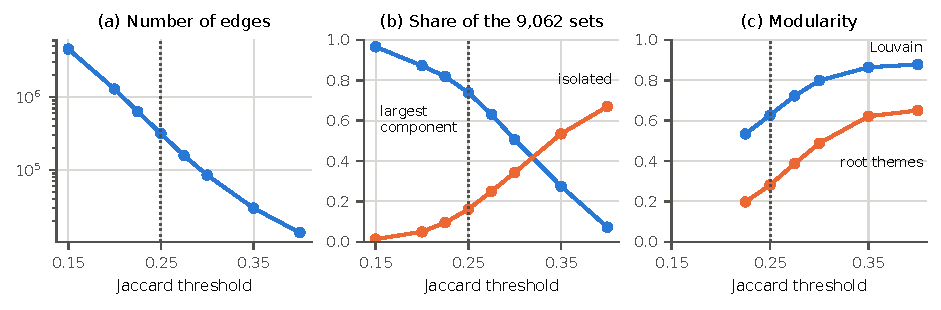
\includegraphics[width=\textwidth]{figures/sensitivity.pdf}
  \caption{Effect of the Jaccard threshold (dotted line: the chosen value
  0.25). (a)~Number of edges, log scale. (b)~Share of sets in the largest
  component and isolated. (c)~Modularity of the Louvain partition and of the
  root themes; Louvain was not run below 0.225 (graph too dense).}
  \label{fig:sensitivity}
\end{figure}

\subsection{Graph statistics}

Table~\ref{tab:stats} summarises the projected graph. It is sparse (density
0.008) but each set has on average 70 neighbours. The degree distribution is
heavy-tailed but bends down on a log--log scale and stops near 1,000
(Figure~\ref{fig:degree}a), so it is not a power law. On the part side
(Figure~\ref{fig:degree}b), 77\% of the parts appear in a single root theme,
while 51 parts appear in 100 themes or more (the 1$\times$2 plate is in 73\% of the
sets).

\begin{table}[htbp]
  \centering
  \small
  \caption{Statistics of the projected set graph (threshold 0.25). $^{*}$On the largest component.}
  \label{tab:stats}
  \begin{tabular}{lr@{\quad}lr}
    \toprule
    Nodes (sets) & 9,062 & Connected & no \\
    Edges & 317,495 & Components & 1,640 \\
    Density & 0.0077 & Isolated sets & 1,462 (16\%) \\
    Mean degree & 70.1 & Largest component & 6,694 sets (74\%) \\
    Maximum degree & 997 & Second component & 282 sets (Duplo) \\
    Median edge weight & 0.27 & Diameter / radius$^{*}$ & 16 / 8 \\
    Mean weighted clustering & 0.14 & Mean distance$^{*}$ & $\approx 3.8$ \\
    \bottomrule
  \end{tabular}
\end{table}

\begin{figure}[htbp]
  \centering
  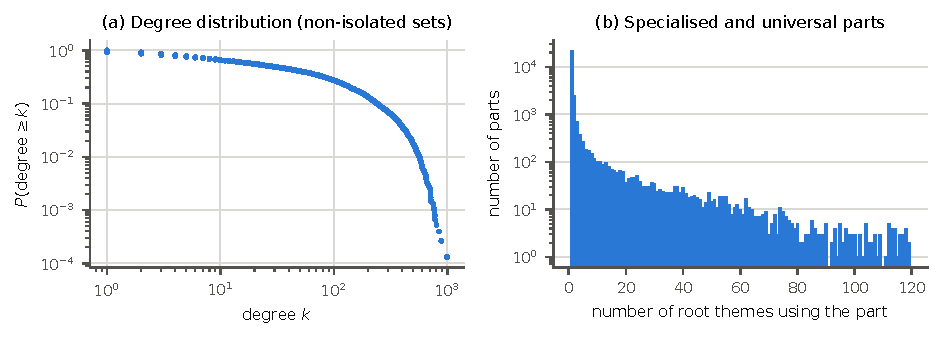
\includegraphics[width=\textwidth]{figures/degree_parts.pdf}
  \caption{(a)~Complementary cumulative degree distribution of the set graph.
  (b)~Number of parts according to the number of root themes in which they
  appear (bipartite graph, log scale).}
  \label{fig:degree}
\end{figure}

\section{Description of the Analysis}
\label{sec:methods}

In short, the analysis has four steps: we describe the graph (connectivity,
distances, central sets), we look for groups of sets that share many parts
(communities), we compare these groups with the official themes, and we check
against random graphs that what we see is not due to chance. We then repeat
the main measures decade by decade.

\paragraph{Software.} The analysis is written in Python 3.11 with NetworkX
3.7 \cite{hagberg2008}, pandas, NumPy, SciPy, scikit-learn
\cite{pedregosa2011} and matplotlib. The projection is computed with sparse
matrices. Exact package versions are frozen in \texttt{uv.lock}, every random
step uses the seed 42, and the README of the repository lists the commands
that produce each table and figure; the figures of this report are drawn from
the result files by \nolinkurl{report/make_figures.py}. The Gephi images (Figure~\ref{fig:gephi}) were made with Gephi
\cite{bastian2009}.

\paragraph{Connectivity and distances.} We compute the connected components.
Since the graph is not connected, the diameter and the radius are computed on
the largest component only, with the exact bounding algorithm of NetworkX
(\texttt{usebounds=True}) \cite{takes2011}. Distances count edges (unweighted):
a path is a chain of sets that pairwise share at least a quarter of their
parts. The mean distance is estimated from 200 random sources. The weighted
clustering coefficient is the weighted version of NetworkX.

\paragraph{Centrality.} We use four measures, each answering a different
question about a set. The \emph{degree} counts the sets that share at least a
quarter of their parts with it, and the \emph{strength} sums the weights of
these links: both tell how ``generic'' a set's parts are. The
\emph{betweenness} \cite{brandes2001} counts how often a set lies on shortest
paths between other sets; it identifies sets that bridge otherwise distant
regions of the catalogue. Since a strong similarity should mean a short
distance, the length of an edge is $1/w$; the measure is
estimated from 500 random sources. The weighted
\emph{eigenvector} centrality, computed on the largest
component, is high for sets connected to other well-connected sets, i.e.\ the
core of the graph.

\paragraph{Communities.} We run the weighted Louvain algorithm
\cite{blondel2008} (resolution 1, seed 42), which maximises the modularity
\cite{newman2004}
\begin{equation}
  Q = \frac{1}{2m}\sum_{i,j}\left(w_{ij} - \frac{s_i s_j}{2m}\right)\delta(c_i, c_j),
\end{equation}
where $s_i$ is the strength of set $i$ and $2m$ the sum of all strengths. We
compare the partition found with the root themes in two ways: the modularity
of the theme partition itself, against two baselines (themes shuffled at
random among sets with the same sizes, and a partition by decade), and the
normalised mutual information (NMI) and adjusted Rand index
(ARI) between communities and themes. The 1,462 isolated sets
each form a one-set community, which inflates the NMI, so we also report NMI
and ARI without them. To check that the conclusion does not depend on the
algorithm, we rerun Louvain at resolutions 0.5, 2 and 4 and run label
propagation \cite{raghavan2007}, in its asynchronous weighted version and in
its deterministic semi-synchronous version. The modularity
of all these partitions is evaluated at resolution 1 so that the values are
comparable.

\paragraph{Cohesion of a theme.} For a theme $t$, let $W_t$ be the total weight
of the edges inside $t$ and $\mathrm{vol}(t)$ the sum of the strengths of its
sets. The \emph{cohesion} (internal share)
\begin{equation}
  c_t = \frac{2W_t}{\mathrm{vol}(t)}
\end{equation}
is the share of the theme's link weight that stays inside the theme: 1 for a
closed universe, close to 0 for a label. If links ignored themes, the expected
value would be $\mathrm{vol}(t)/2m$. We report it for the 57 root themes with
at least 30 sets.

\paragraph{Null model.} A theme can look cohesive only because its sets are
large or contain frequent parts. To control for this, we shuffle the bipartite
sets $\times$ parts matrix with the curveball algorithm \cite{strona2014}: it
repeatedly picks two sets and redistributes the parts they do not share. Every
set keeps exactly its number of parts and every part its number of sets; only
the link between parts and themes is destroyed. After 20 rounds, 22\% of the
set--part pairs are still in place. We draw 10 null matrices (seeds 42 to 51)
and project each of them. At the threshold 0.25 a null graph has almost no
edges (117 to 235), so we keep its strongest edges, as many as in the real
graph (cut-off $\approx 0.16$), and compute the same cohesion. With 10 draws
the smallest possible empirical p-value is $1/11 \approx 0.09$, so we report
how many draws reach the real value and the ratio between the real cohesion
and its mean in the null graphs.

\paragraph{Theme graph and theme prediction.} We contract the set graph into a
graph of the 127 root themes: the weight of the edge between themes $a$ and
$b$ is the total weight $W_{ab}$ of the links between their sets, and its
\emph{lift} $W_{ab} / (\mathrm{vol}(a)\,\mathrm{vol}(b)/2m)$ compares it with
the weight expected if links ignored themes (lift $>1$: more linked than
chance). We also ask whether a set's neighbours reveal its theme: each
neighbour votes for its own root theme with the weight of the edge, the set's
own theme is never used, and isolated sets get no prediction. We compare the
success rate with always predicting the most frequent theme and with drawing a
theme at random according to the theme frequencies.

\paragraph{Evolution over time.} We rebuild the graph separately for 1990--1999,
2000--2009, 2010--2019 and 2020--2025 and recompute the modularity of the
themes, Louvain and the NMI. Specialisation is measured on the bipartite graph,
independently of the threshold: for a set, the \emph{exclusive share} is the
share of its distinct parts that appear in no other root theme of the
1990--2025 catalogue; we also report the number of exclusive parts per set and
the number of distinct parts per set. Because a sticker sheet is a part number
specific to one set, we repeat the analysis without the Rebrickable category
``Stickers'', and at the thresholds 0.25 and 0.35.

\paragraph{Reused code and AI tools.} No existing code analysing the
Rebrickable data was reused. Graph algorithms (components, diameter,
centralities, Louvain, label propagation, modularity) come from NetworkX, and
NMI and ARI from scikit-learn; the curveball algorithm was implemented by us
from its description in \cite{strona2014}. We used Claude Code (Anthropic), an
AI coding assistant, to help write and test the analysis code, to search for
related studies, and to draft and format this report. All numbers in the
report are produced by the scripts of the repository, and we checked the
modelling choices and the interpretations ourselves.

\section{Results}
\label{sec:results}

\subsection{Connectivity, distances and central sets}

The graph is not connected (Table~\ref{tab:stats}). The largest component
holds 74\% of the sets; 16\% of the sets share at least a quarter of their
parts with no other set and are isolated. The second component (282 sets) is
almost entirely Duplo (216 sets) and Duplo-based educational sets: Duplo
bricks are not compatible in size with the rest of the catalogue, and the graph
shows it as a separate island. Smaller components are also single themes:
LEGO Brand Store (23 sets), Clikits (21), Belville (12). Inside the largest
component, any two sets are at most 16 steps apart and about 3.8 steps on
average. The eight sets of the center (eccentricity 8) are large models for
adults (Ford Mustang, Volkswagen T2 Camper Van, Land Rover Defender, Voltron,
Tantive~IV); the three sets of the periphery are atypical (a Botanicals flower
bouquet, an educational kit, a 2007 Racers car). The center of the catalogue is
therefore not a theme but a type of set: large, recent, and built from common
parts.

\begin{table}[htbp]
  \centering
  \small
  \caption{Five most central sets for each measure (root theme, year).}
  \label{tab:centrality}
  \begin{tabular}{@{}l@{\ }p{0.8\textwidth}@{}}
    \toprule
    Degree &
    The Brick Moulding Machine (LEGO Exclusive, 2021) 997;
    R2-D2 (Star Wars, 2021) 885;
    Luke Skywalker's Landspeeder (Star Wars, 2022) 847;
    Old Trafford -- Manchester United (Creator, 2020) 803;
    The Dark Falcon (Star Wars, 2024) 783 \\
    \addlinespace
    Betweenness &
    Architecture Studio (Architecture, 2013) 0.037;
    Fallingwater (Architecture, 2009) 0.030;
    NANO QUEST Challenge Kit (FIRST LEGO League, 2006) 0.024;
    Amusement Park (Factory, 2005) 0.018;
    Skyline (Factory, 2005) 0.016 \\
    \addlinespace
    Eigenvector &
    The Dark Falcon (Star Wars, 2024) 0.070;
    Ghost \& Phantom II (Star Wars, 2023) 0.070;
    R2-D2 (Star Wars, 2021) 0.070;
    Luke Skywalker's Landspeeder (Star Wars, 2022) 0.070;
    Jazz Quartet (LEGO Ideas, 2022) 0.068 \\
    \bottomrule
  \end{tabular}
\end{table}

The centralities (Table~\ref{tab:centrality}) tell the same story. The sets
with the highest degree and strength (the order is almost the same for both)
are large display models from 2019--2024, mostly Star Wars, which use a wide
range of standard parts and thus resemble hundreds of other sets. Eigenvector
centrality concentrates on the same group: recent large Star Wars, Ideas,
Marvel and DC sets form the densest core of the graph. Betweenness highlights a
different kind of set: bridges whose inventory mixes part families. Architecture
Studio is a box of white and transparent bricks of all kinds, the FIRST LEGO
League kits combine Technic and classic bricks, and the 2005 Factory sets were
designed from fan models with unusual part assortments. A theme like Star Wars
is central because it is large and generic, not because it is a hub of
specific parts.

\subsection{Communities are not themes}

\begin{table}[htbp]
  \centering
  \small
  \caption{Partitions of the set graph compared with the root themes.
  Modularity is always evaluated at resolution 1; NMI and ARI exclude the
  1,462 isolated sets. ``$\geq 10$'': number of groups with at least 10 sets;
  ``largest'': share of the sets in the largest group.}
  \label{tab:communities}
  \setlength{\tabcolsep}{4.5pt}
  \begin{tabular}{lrrrrr}
    \toprule
    Partition & $\geq 10$ & largest & modularity & NMI & ARI \\
    \midrule
    Root themes (127) & 87 & 8\% & 0.282 & 1 & 1 \\
    Root themes shuffled at random & 87 & 8\% & 0.000 & -- & -- \\
    Decades (4) & 4 & 38\% & 0.360 & -- & -- \\
    \midrule
    Louvain, resolution 0.5 & 24 & 22\% & 0.610 & 0.43 & 0.10 \\
    Louvain, resolution 1 & 35 & 19\% & 0.627 & 0.45 & 0.10 \\
    Louvain, resolution 2 & 39 & 12\% & 0.588 & 0.49 & 0.15 \\
    Louvain, resolution 4 & 59 & 7\% & 0.477 & 0.54 & 0.22 \\
    Label propagation, asynchronous & 32 & 27\% & 0.580 & 0.49 & 0.09 \\
    Label propagation, semi-synchronous & 36 & 28\% & 0.577 & 0.47 & 0.08 \\
    \bottomrule
  \end{tabular}
\end{table}

Louvain finds 1,677 communities, of which 1,462 are isolated sets and only 35
have at least 10 sets, with a modularity of 0.63 (Table~\ref{tab:communities}).
The theme partition reaches only 0.28. This is far above shuffled themes
($\approx 0$), so themes do structure the graph, but much less than the best
partition. The agreement between communities and themes is moderate
(NMI 0.45 without isolated sets) and the ARI is low (0.10).
Figure~\ref{fig:heatmap} shows why. The four largest communities, which
together hold more than half of the sets, are mixtures of themes from the same period:
community C1 (median year 2004) mixes Town, Star Wars, Creator and Space, C3
(2016) mixes City, Star Wars, Friends and Ninjago, and C2 (2023) Friends,
Star Wars, Marvel and City. Only the themes with their own building system
form their own community: Technic (C4, 66\% Technic, with Bionicle and Racers,
which use Technic parts) and Duplo (C6, 81\% Duplo). The Gephi drawing of the
graph (Figure~\ref{fig:gephi}) gives the same picture: the colour patches of
the communities cut across the colours of the themes.

At the threshold 0.25, the partition by decade even has a higher modularity
than the themes (0.36 against 0.28). This comparison, however, depends on the
threshold: at 0.30 the themes are ahead (0.49 against 0.43) and at 0.35 clearly
so (0.62 against 0.48), because a higher threshold keeps only very similar
sets, which tend to belong to the same theme (these two values are computed by
\nolinkurl{report/extra_checks.py}). We therefore do not claim that
time structures the catalogue more than themes; we only conclude that large
communities group sets by period rather than by theme.

The conclusion does not depend on the algorithm. Label propagation gives
partitions close to Louvain (NMI 0.47--0.49, modularity 0.58). Increasing the
Louvain resolution raises the NMI from 0.43 to 0.54 and the ARI from 0.10 to
0.22: at resolution 4 the giant mixed communities break up (the largest goes
from 22\% to 7\% of the sets) and the granularity becomes close to that of the
themes. Even then, the ARI stays at 0.22, far from a match.

\begin{figure}[htbp]
  \centering
  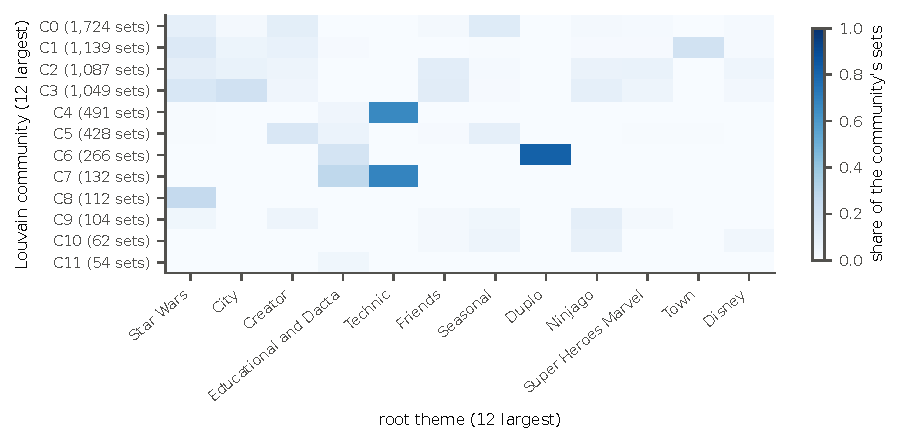
\includegraphics[width=\textwidth]{figures/communities_heatmap.pdf}
  \caption{Composition of the 12 largest Louvain communities in terms of the
  12 largest root themes (share of the community's sets; columns do not sum to
  1 because other themes are omitted).}
  \label{fig:heatmap}
\end{figure}

\begin{figure}[htbp]
  \centering
  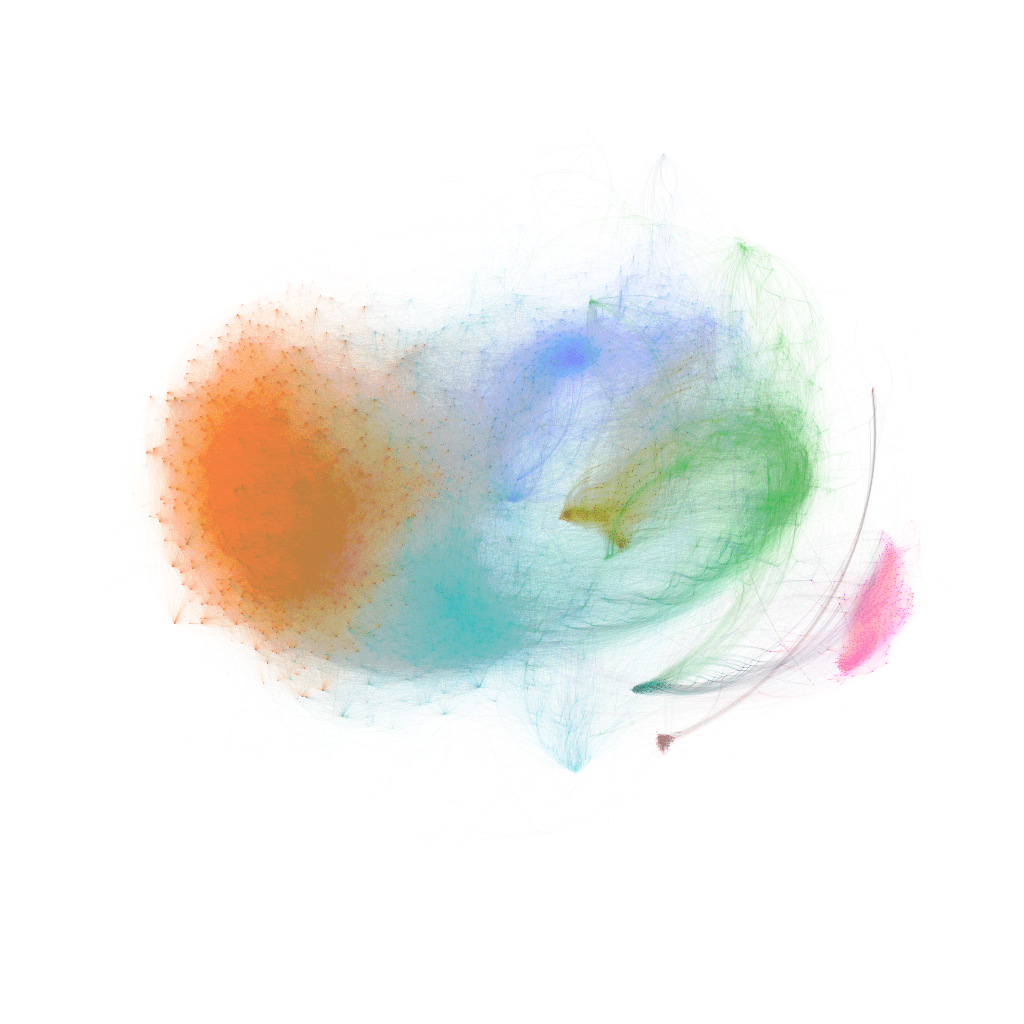
\includegraphics[width=0.4\textwidth]{figures/gephi_communities.png}
  \hspace{0.04\textwidth}
  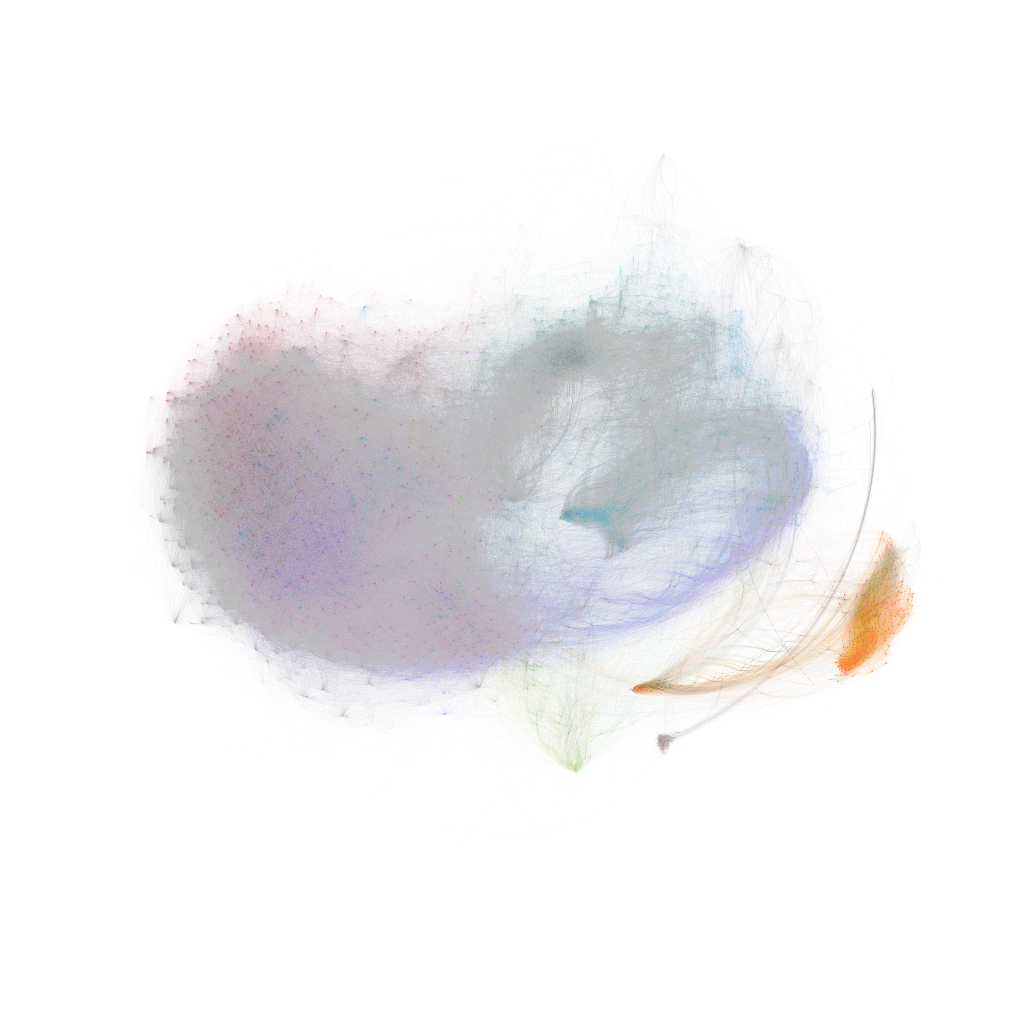
\includegraphics[width=0.4\textwidth]{figures/gephi_root_themes.png}
  \caption{The set graph drawn with Gephi (ForceAtlas2 layout,
  isolated sets removed, same layout in both panels). Left: coloured by
  Louvain community; right: coloured by root theme. Colours come from Gephi's
  partition palette, in which many small themes get similar colours: the
  figure is meant for the overall comparison, not to identify single themes.}
  \label{fig:gephi}
\end{figure}

\subsection{Which themes are universes?}

\begin{figure}[htbp]
  \centering
  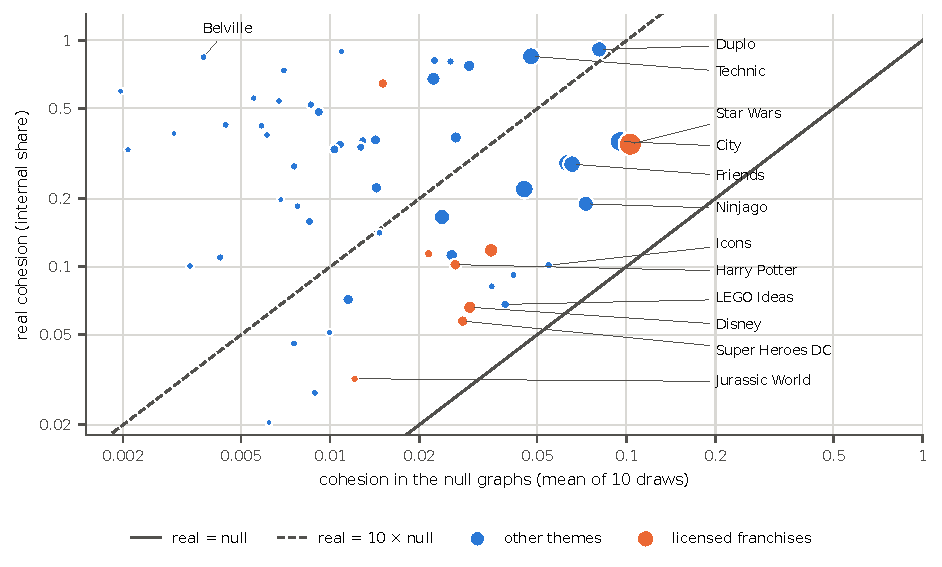
\includegraphics[width=\textwidth]{figures/cohesion_null.pdf}
  \caption{Cohesion of the 57 root themes with at least 30 sets, against their
  mean cohesion in 10 null graphs (log scales; point size: number of sets).
  All themes lie above the line ``real = null''; most licensed franchises lie
  between the two lines, i.e.\ less than 10 times above chance.}
  \label{fig:cohesion}
\end{figure}

\begin{table}[htbp]
  \centering
  \small
  \caption{Selected root themes: number of sets, cohesion $c_t$, mean
  cohesion in the null graphs and ratio, and theme prediction by neighbour
  vote (recall: share of the theme's linked sets correctly guessed; precision:
  share of the predictions of this theme that are correct).}
  \label{tab:themes}
  \begin{tabular}{lrrrrrr}
    \toprule
    Root theme & sets & cohesion & null & ratio & recall & precision \\
    \midrule
    Duplo & 339 & 0.91 & 0.081 & 11.3 & 0.88 & 0.82 \\
    Technic & 419 & 0.85 & 0.048 & 17.8 & 1.00 & 0.75 \\
    Brickheadz & 181 & 0.77 & 0.029 & 26.2 & 1.00 & 0.46 \\
    Town & 246 & 0.68 & 0.022 & 30.3 & 0.93 & 0.82 \\
    Castle & 102 & 0.48 & 0.009 & 52.6 & 0.92 & 0.92 \\
    City & 582 & 0.36 & 0.095 & 3.7 & 0.76 & 0.90 \\
    Star Wars & 721 & 0.35 & 0.103 & 3.4 & 0.86 & 0.41 \\
    Friends & 402 & 0.28 & 0.066 & 4.3 & 0.83 & 0.62 \\
    Creator & 457 & 0.22 & 0.045 & 4.9 & 0.57 & 0.39 \\
    Ninjago & 331 & 0.19 & 0.073 & 2.6 & 0.59 & 0.76 \\
    Super Heroes Marvel & 266 & 0.12 & 0.035 & 3.4 & 0.40 & 0.66 \\
    Harry Potter & 159 & 0.10 & 0.026 & 3.9 & 0.45 & 0.76 \\
    Disney & 216 & 0.07 & 0.030 & 2.2 & 0.33 & 0.82 \\
    Super Heroes DC & 152 & 0.06 & 0.028 & 2.1 & 0.11 & 0.50 \\
    Jurassic World & 65 & 0.03 & 0.012 & 2.6 & 0.17 & 0.67 \\
    LEGO Ideas & 92 & 0.07 & 0.039 & 1.7 & 0.00 & 0.00 \\
    \bottomrule
  \end{tabular}
\end{table}

The cohesion of the 57 themes with at least 30 sets ranges from 0.03 to 0.91
(median 0.29; Table~\ref{tab:themes}). At the top are themes with a dedicated
building system or a strong visual style: Duplo (0.91), Clikits (0.89),
Technic (0.85), Belville (0.84), Mixels and DOTS (0.81), Brickheadz (0.77).
At the bottom are licensed franchises and catch-all themes: Harry Potter
keeps only 10\% of its link weight inside the theme, Disney 7\%, Super Heroes
DC 6\%, Jurassic World 3\%.

The null model qualifies the reading of these low values
(Figure~\ref{fig:cohesion}). When parts are shuffled between sets, the
modularity of the themes falls from 0.28 to 0.004--0.005, and \emph{all 57
themes are more cohesive than in each of the 10 null graphs}. Most themes are far above chance (median ratio 19), especially those with
their own parts such as Castle, Town or Technic. Film franchises are only 2 to
4 times above chance (Harry Potter, Marvel, Disney, DC, Jurassic World), and
the theme closest to chance, LEGO Ideas, is by design a collection of fan
projects with no common world. Minecraft is the exception among licences: its
sets use dedicated block-shaped parts. Note that the ratio is lower for large
themes, whose cohesion is already high by chance, which is why Star Wars and
City have a ratio close to the film franchises although they are much more
cohesive. Film franchises are therefore not mere labels, but \emph{weak
universes}: their sets share a little more than chance, much less than Technic
or Duplo.

The theme graph (Figure~\ref{fig:themegraph}) shows how themes relate. It has
127 nodes and 2,487 edges (density 0.31); 7 small themes (2 to 19 sets) have no
link at all. The heaviest edges go through the two largest generic themes,
Creator--Star Wars (6,942 links between sets) and Star Wars--Icons, but their
lift is close to 1 (1.10 and 1.38): they are heavy only because both themes are
large. The lift reveals families instead: Castle--Pirates (56),
Pirates--Adventurers (45), Train--Town (20) and Bionicle--Hero Factory (15)
are themes of the same period or the same part system; Hero Factory replaced
Bionicle in 2010.

The prediction experiment confirms the picture. Voting among neighbours
guesses the root theme of 63.9\% of the 7,600 linked sets (61.6\% without
weights; 53.6\% if isolated sets count as failures), against 8.4\% by always
predicting Star Wars and 3.1\% at random. Averaged over the 57 large themes,
the success rate is 59\%. Recall is highest for the closed universes (Technic
and Brickheadz 100\%, Town 93\%, Castle 92\%, Duplo 88\%) and lowest for the
licensed and catch-all themes (DC 11\%, Jurassic World 17\%, LEGO Ideas 0\%),
whose sets are mostly predicted as Star Wars. Recall alone can be misleading:
Star Wars is guessed for 86\% of its sets, but it is predicted for 1,337 sets
of which only 41\% are Star Wars. As the largest theme with generic parts, it
attracts the vote of its neighbours (most of its false predictions are Creator,
Marvel, Ninjago and DC sets). Brickheadz shows the same effect (precision
0.46): it absorbs Seasonal and Promotional sets built in the same style.

\begin{figure}[htbp]
  \centering
  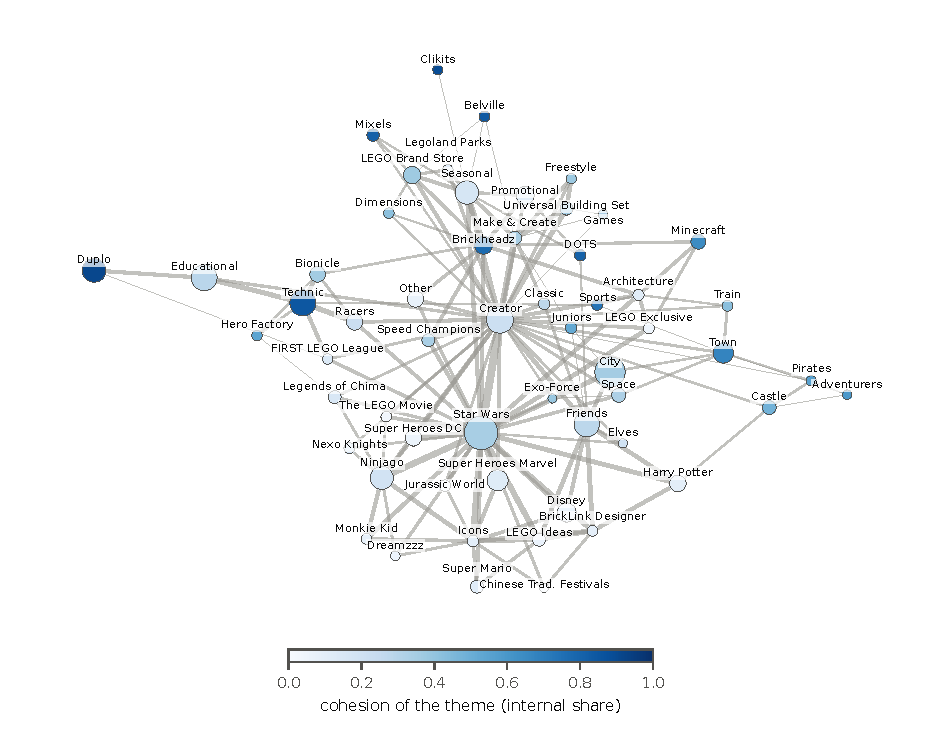
\includegraphics[width=\textwidth]{figures/theme_graph.pdf}
  \caption{Theme graph: one node per root theme with at least 30 sets (size:
  number of sets; colour: cohesion $c_t$), with the 3 heaviest edges of each
  theme (width: total Jaccard weight between the two themes).}
  \label{fig:themegraph}
\end{figure}

\subsection{Did LEGO become more specialised?}

\begin{table}[htbp]
  \centering
  \small
  \caption{Evolution by period. Modularity of the root themes at thresholds
  0.25 and 0.35; exclusive parts with stickers kept (removed in brackets).
  Exclusive parts do not depend on the threshold.}
  \label{tab:temporal}
  \begin{tabular}{lrrrrrrr}
    \toprule
    & & & \multicolumn{2}{c}{modularity} & \multicolumn{2}{c}{exclusive parts} & parts \\
    \cmidrule(lr){4-5} \cmidrule(lr){6-7}
    Period & sets & themes & 0.25 & 0.35 & share & per set & per set \\
    \midrule
    1990--1999 & 927 & 30 & 0.52 & 0.54 & 8.9\% (8.3\%) & 4.6 (4.2) & 57 \\
    2000--2009 & 1,780 & 57 & 0.31 & 0.47 & 9.0\% (8.4\%) & 4.2 (3.9) & 61 \\
    2010--2019 & 3,411 & 70 & 0.32 & 0.67 & 4.4\% (3.9\%) & 2.9 (2.4) & 79 \\
    2020--2025 & 2,944 & 56 & 0.17 & 0.62 & 4.4\% (4.0\%) & 3.8 (3.3) & 103 \\
    \bottomrule
  \end{tabular}
\end{table}

\begin{figure}[htbp]
  \centering
  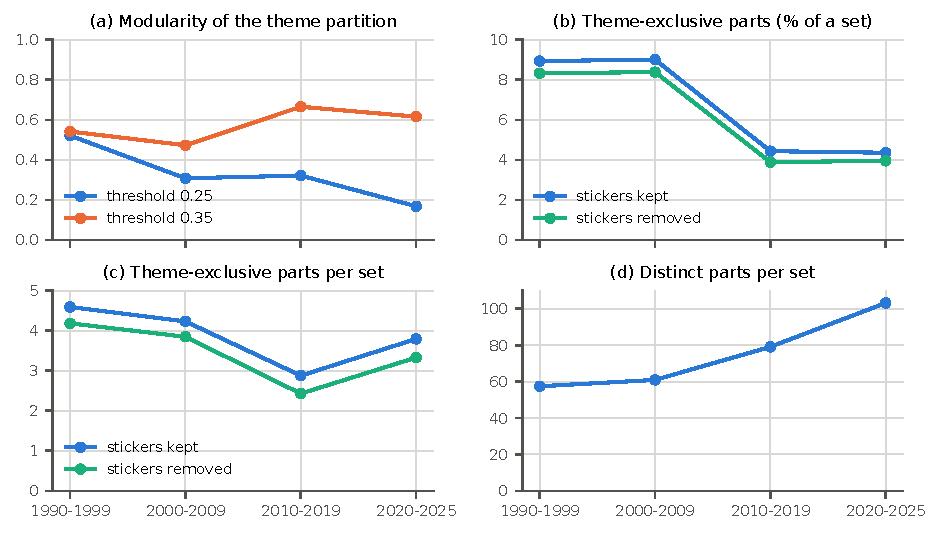
\includegraphics[width=\textwidth]{figures/temporal.pdf}
  \caption{Evolution by period. (a)~Modularity of the root themes at two
  thresholds. (b)~Share and (c)~number of a set's parts that appear in no other
  root theme, with and without stickers. (d)~Mean number of distinct parts per
  set.}
  \label{fig:temporal}
\end{figure}

Our hypothesis was that sets became more theme-specific after 2000. The data
do not support it (Table~\ref{tab:temporal}, Figure~\ref{fig:temporal}). The
share of a set's parts that no other theme uses stays at 9\% in the 1990s and
2000s, then halves to 4.4\% in the 2010s and 2020s. This result does not
depend on the threshold, which only affects the projection, and it is not
caused by stickers: without them the share goes from 8.3\% to 4.0\%. It also
holds under other modelling choices (minimum set size of 20 or 100 parts,
parts distinguished by colour, no excluded theme, parts present in more than
20\% of the sets removed): in every case the share in the 2010s and 2020s
(3.8--6.4\%) is about half of the share in the 1990s (8.5--11.7\%).

The counts explain this decline. The number of exclusive parts per set falls
less (4.6 in the 1990s, 2.9 in the 2010s) and rises again in the 2020s (3.8),
while sets grow from 57 to 103 distinct parts on average. Sets have become
larger, as Bartneck and Moltchanova found \cite{bartneck2018}, but the parts
they added are mostly parts shared across themes. Their conclusion that sets
became more specialised is about the growing vocabulary of the catalogue; at
the level of themes, we find the opposite: a smaller share of each set is
specific to its theme.

The structural indicators are less conclusive. At the threshold 0.25, the
modularity of the themes falls from 0.52 to 0.17 and the NMI between Louvain
communities and themes from 0.70 to 0.42, which would suggest that themes are
melting into each other. But at 0.35 the modularity of the themes rises
instead (0.54, 0.47, 0.67, 0.62). Recent sets are larger and share more
standard parts, so at a fixed threshold they get many more links (39 links per
set in the 2010s, 79 in the 2020s, against 24 in the 1990s), and the
modularity at 0.25 partly measures this density. We therefore do not report a
trend in modularity, only the robust decline of theme-exclusive parts.

\section{Conclusions}
\label{sec:conclusion}

LEGO themes are, for the most part, not separate universes. Sets mainly link
to sets of the same period, and the communities of the graph mix themes of the
same era (NMI 0.45 with the themes, ARI 0.10, whatever the algorithm). Only a
few themes are closed worlds, those with their own building system or style:
Duplo, Technic, Clikits, Belville, Brickheadz. Film franchises such as Harry
Potter, Marvel, DC, Disney and Jurassic World are weak universes: only 3 to
12\% of their link weight stays inside the theme, but they remain 2 to 4 times
more cohesive than chance, and all 57 large themes beat all ten null graphs. Over time, LEGO did not become more theme-specific:
the share of theme-exclusive parts in a set halved between the 2000s and the
2010s, because sets grew with parts shared across the catalogue. Centrality
measures point in the same direction: the most central sets are large, recent,
generic models, and the bridges are sets that mix part families.

\paragraph{Limitations.} The projection depends on the threshold. We only
draw conclusions that hold from 0.25 to 0.35; the comparison between themes
and decades, and the trend of modularity over time, do not, and are not
claimed. A printed part or a sticker sheet has its own part number, which
inflates exclusive parts; removing stickers changes little, but printed parts
are still counted separately. Rebrickable is maintained by volunteers, and we
use only the first version of each inventory and ignore minifigures. The null
model uses 10 draws, so p-values cannot go below 0.09, and it is compared at
equal density rather than at the same threshold. The projection discards part
of the bipartite structure \cite{barber2007}. Finally, Louvain and
asynchronous label propagation depend on the seed and, for near-ties, on the
machine: on a second computer, with the same code and versions, the NMI of
2000--2009 was 0.52 instead of 0.53.

\paragraph{Future work.} Community detection directly on the bipartite graph
\cite{barber2007} would avoid the threshold altogether. Weighting parts by
quantity or by colour, adding minifigures, and studying the graph of parts
(which parts are used together) would refine the notion of a theme's own
parts. More null draws would give proper p-values.

{\small
\bibliographystyle{plain}
\bibliography{biblio}
}

\end{document}
